\documentclass{beamer}
\usepackage[utf8]{inputenc}
\usepackage{amsmath}
\usepackage{amsfonts}
\usepackage{amssymb}
\usepackage{makeidx}
\usepackage{graphicx}
\usepackage{lmodern}
\usepackage{color}
\usepackage{xcolor}
\usepackage{bussproofs}
\usepackage{lscape}
\usepackage{listings}
\usepackage{amsthm}
\usetheme{CambridgeUS}
\usepackage{booktabs}
\usefonttheme{serif}

\title{PDL SAT solver}
\author{Mudathir Mahgoub}
  
 
\begin{document}
 
\frame{\titlepage}
 
\begin{frame}
\frametitle{Project problem}
Given a formula in propositional dynamic logic (PDL), and optionally a kripke frame, is this formula satisfiable?
\end{frame}

\begin{frame}[fragile]
\frametitle{Execution}
\scriptsize

\begin{block}{Input: test.pdl}
\begin{verbatim}
(p and q) and
<do p -> a | q -> b od>
    (
        (<b> (p and not q))  and
        (<a> (q and not p))
    )
\end{verbatim}
Which is equivalent to :
\begin{align*}
((p \wedge q) \wedge \langle\textbf{ do }p \rightarrow a \vert q \rightarrow b\textbf{ od }\rangle(\langle b\rangle(p \wedge \neg q) \wedge \langle a \rangle(q \wedge \neg p)))
\end{align*}
\end{block}
\end{frame}


\begin{frame}[fragile]
\frametitle{Execution}
\begin{block} {Output: java -jar pdl.jar -i test.pdl}
\small
\begin{lstlisting} 
K = {0, 2, 1, 3}
m(p) = {0, 3}
m(q) = {1, 3}
m(a) = {(2,1), (3,2)}
m(b) = {(2,0)}
Satisfying states: [3]
\end{lstlisting} 
\end{block}
\end{frame}

\begin{frame}[fragile]
\frametitle{Execution}
\huge
\centering

Demo

\end{frame}

\begin{frame}[fragile]
\frametitle{Problem complexity}
\begin{block}{Without a kripke frame}
\begin{itemize}
\item The problem is decidable and it is \textit{EXPTIME-complete}
\item Satisfiability problem in propositional logic is \textit{NP-complete}
\item We don't know whether $NP = EXPTIME$
 \vfill 
\end{itemize}

 \vfill 

\end{block}
\begin{block}{With kripke frame}
\begin{itemize}
\item The problem is in $P$
\item Can be solved using graph algorithms like DFS
\end{itemize}
\end{block}
\end{frame}


\begin{frame}
\frametitle{Software components}
\begin{figure}
 \centering
 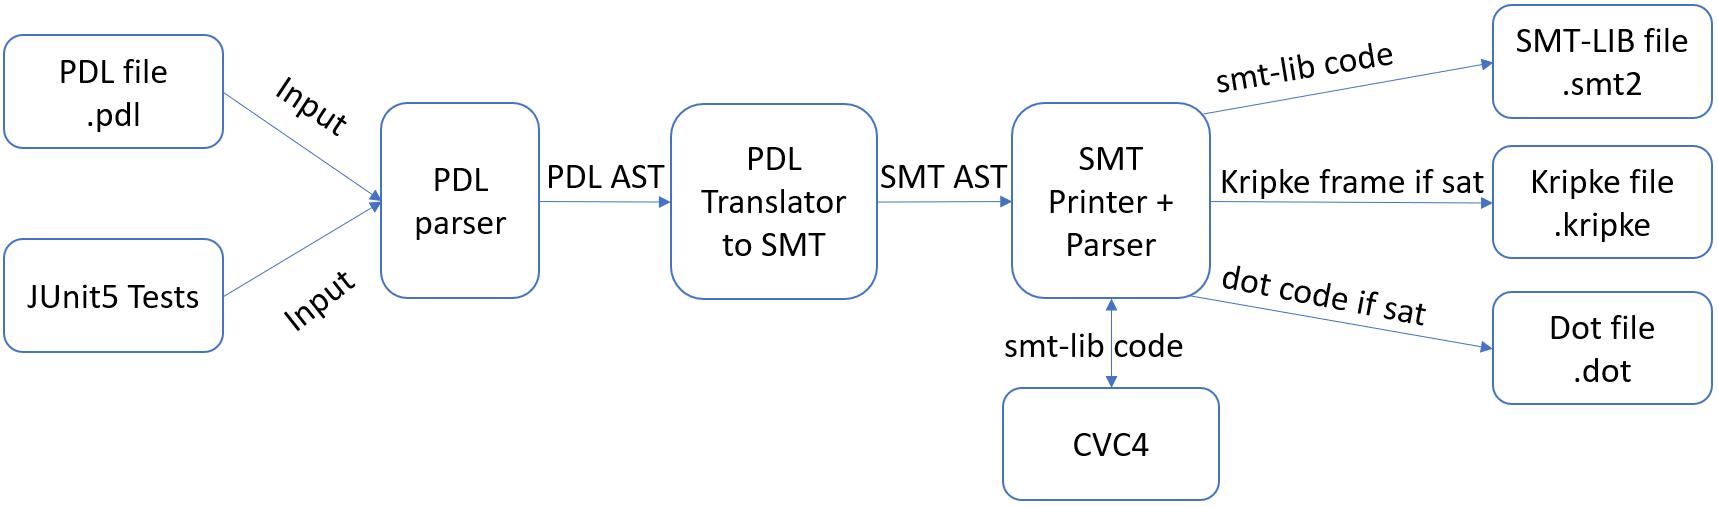
\includegraphics[scale=.25,keepaspectratio=true]{./solver.png}
\end{figure}
\end{frame}



\begin{frame}
\frametitle{CVC4 Overview}

\begin{itemize}
\item Automatic theorem prover for satisfiability modulo theories (SMT) problems
 \vfill 
\item Can be used to prove the validity (or the satisfiability) of first-order formulas in many logical theories and their combination

\end{itemize}
\end{frame}

\begin{frame}[fragile]
\frametitle{CVC4 Overview}
\huge
\centering

Demo

\end{frame}



\begin{frame}[fragile]
\frametitle{PDL Translation to CVC4}
\begin{tabular}{ll} 
\toprule
PDL & CVC4 \\    
\midrule    
$K=\lbrace u_0, u_1, \cdots u_n \rbrace$ &  
$\begin{matrix}
\text{\textbf{Atom} : \text{Uninterpreted sort}} \\
u_0, u_1, \cdots, u_n: \textbf{Atom} \\
\textit{atomUniverse} = \lbrace \langle u_0 \rangle, \langle u_1 \rangle, \cdots , \langle u_n \rangle \rbrace \\
\textit{atomIdentity}:  = \lbrace \langle u_0, u_0 \rangle, \langle u_1, u_1 \rangle, \cdots , \langle u_n, u_n \rangle \rbrace \\
\end{matrix}$ \\ \bottomrule
\end{tabular}
\end{frame} 

\begin{frame}[fragile]
\frametitle{PDL Translation to CVC4}
\begin{tabular}{ll} 
\toprule
PDL & CVC4 \\    
\midrule   

\textbf{0} & \textit{emptyset} : (Set (Tuple \textbf{Atom})) \\
\textbf{1} & \textit{atomUniverse} \\
Atomic propositions $p, q, r, \cdots$ & $p, q, r, \cdots : \text{Set(Tuple (\textbf{Atom}))}$ \\
Atomic programs $a, b, c, \cdots$ & $a, b, c \cdots : \text{Set(Tuple (\textbf{Atom}$,$\textbf{Atom}))}$ \\
$p \vee q$ & $p \cup q$ \\
$p \wedge q$ & $p \cap q$ \\
$\neg p$ & $\textit{atomUniverse} - p$ \\
$p \rightarrow q$ & $(\textit{atomUniverse}- p)\cup q$ \\
$a;b$ & $a \circ b$ where $\circ$ is the join operator\\
$a \cup b$ (choice) & $a \cup b$ (union)\\
$a*$ (choice) & $a \cup a^+$, $a^+$ is the transitive closure\\
$p?$ (test) & $(p \times p) \cap \textit{atomIdentity}$\\
\bottomrule
\end{tabular}
\end{frame}

\begin{frame}[fragile]
\frametitle{Satisfiability  validity}

\begin{itemize}
\item When do we say a PDL formula $\varphi$ is satisfiable? \\
\pause
A PDL formula $\varphi$ is satisfiable if its meaning is nonempty in some kripke frame (i.e. $\exists \mathfrak{K} . \; m_{\mathfrak{K}}(\varphi) \neq \phi$). 
\vfill
\item When do we say a PDL formula $\varphi$ is valid in all kripke frames? \\
\pause 
A PDL formula $\varphi$ is valid if  $\forall \mathfrak{K} .(m_{\mathfrak{K}}(\varphi) = K$) \\
Alternatively  \\
A PDL formula $\varphi$ is valid if  $\neg \varphi$ is unsatisfiable in all kripke frames \\
\vfill
\item A PDL formula $\varphi$ is valid in a given Kripke frame $\mathfrak{K}$ if $m(\varphi) = K$ or $m(\neg \varphi) = \phi$)
\end{itemize}

\end{frame}

\begin{frame}[fragile]
\frametitle{Examples}
\small
\begin{align*}
[((a \cup b) \cup c)](q \wedge \neg p)
\end{align*}
\begin{tabular}{ll} 
\begin{lstlisting} 
K = {01,2,3,4,5}
m(p) = {01,2,4}
m(q) = {01,3}
m(r) = {5}
m(a) = {(01,2),(01,4),(2,4),(01,3)}
m(b) = {(01,3),(3,3)}
m(c) = {(5,5)}
\end{lstlisting} &
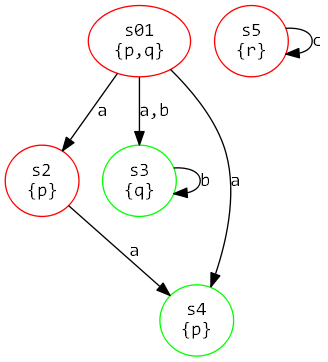
\includegraphics[scale=0.3]{example2.png}
\end{tabular}
\end{frame}

\begin{frame}[fragile]
\frametitle{Examples}
\small
\begin{align*}
\langle \textbf{while } p\textbf{ do }a \rangle p
\end{align*}
Unsat
\begin{align*}
\langle \textbf{while } p\textbf{ do }a \rangle \neg p
\end{align*}
\begin{tabular}{ll} 
\begin{lstlisting} 
K = {0, 1}
m(p) = {1}
m(a) = {(1,0)}
\end{lstlisting} &
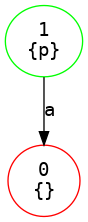
\includegraphics[scale=0.3]{while.png}
\end{tabular}
\end{frame}


\begin{frame}[fragile]
\frametitle{Examples}
Axiom 7 in the Axiom system 5.5
\begin{align*}
p \wedge [a][a*] p \leftrightarrow [a*]p
\end{align*}
Its negation is
\begin{align*}
\neg (p \wedge [a][a*] p \leftrightarrow [a*]p)
\end{align*}
\small
\begin{tabular}{ll} 
\begin{lstlisting} 
K = {0}
m(p) = {}
m(a) = {}
Satisfying states: [0]
\end{lstlisting} &
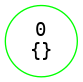
\includegraphics[scale=0.3]{axiom7.png}
\end{tabular}
\end{frame}

\begin{frame}[fragile]
\frametitle{Examples}
Hoare Logic partial correctness assertion

\begin{align*}
\lbrace p \rbrace a \lbrace q \rbrace = p \rightarrow [a] q
\end{align*}
\begin{align*}
\lbrace p \rbrace a \lbrace q \rbrace \wedge  \lbrace q \rbrace b \lbrace r \rbrace
\rightarrow
\lbrace p \rbrace a;b \lbrace r \rbrace
\end{align*}
Counter example
\small
\begin{tabular}{ll} 
\begin{lstlisting} 
K = {0, 1}
m(p) = {0, 1}
m(q) = {1}
m(r) = {0}
m(a) = {(0,1), (1,0)}
m(b) = {(0,1), (1,1)}
Satisfying states: [0]
\end{lstlisting} 
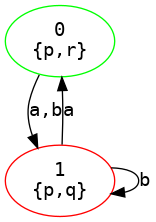
\includegraphics[scale=0.3]{hoare1.png}
\end{tabular}
\end{frame}


\end{document}
